\hypertarget{phonefirewall__administration_8c}{
\section{phonefirewall\_\-administration.c File Reference}
\label{phonefirewall__administration_8c}\index{phonefirewall\_\-administration.c@{phonefirewall\_\-administration.c}}
}
{\tt \#include $<$stdio.h$>$}\par
{\tt \#include $<$stdlib.h$>$}\par
{\tt \#include $<$errno.h$>$}\par
{\tt \#include $<$string.h$>$}\par
{\tt \#include \char`\"{}libphonefirewall.h\char`\"{}}\par


Include dependency graph for phonefirewall\_\-administration.c:\nopagebreak
\begin{figure}[H]
\begin{center}
\leavevmode
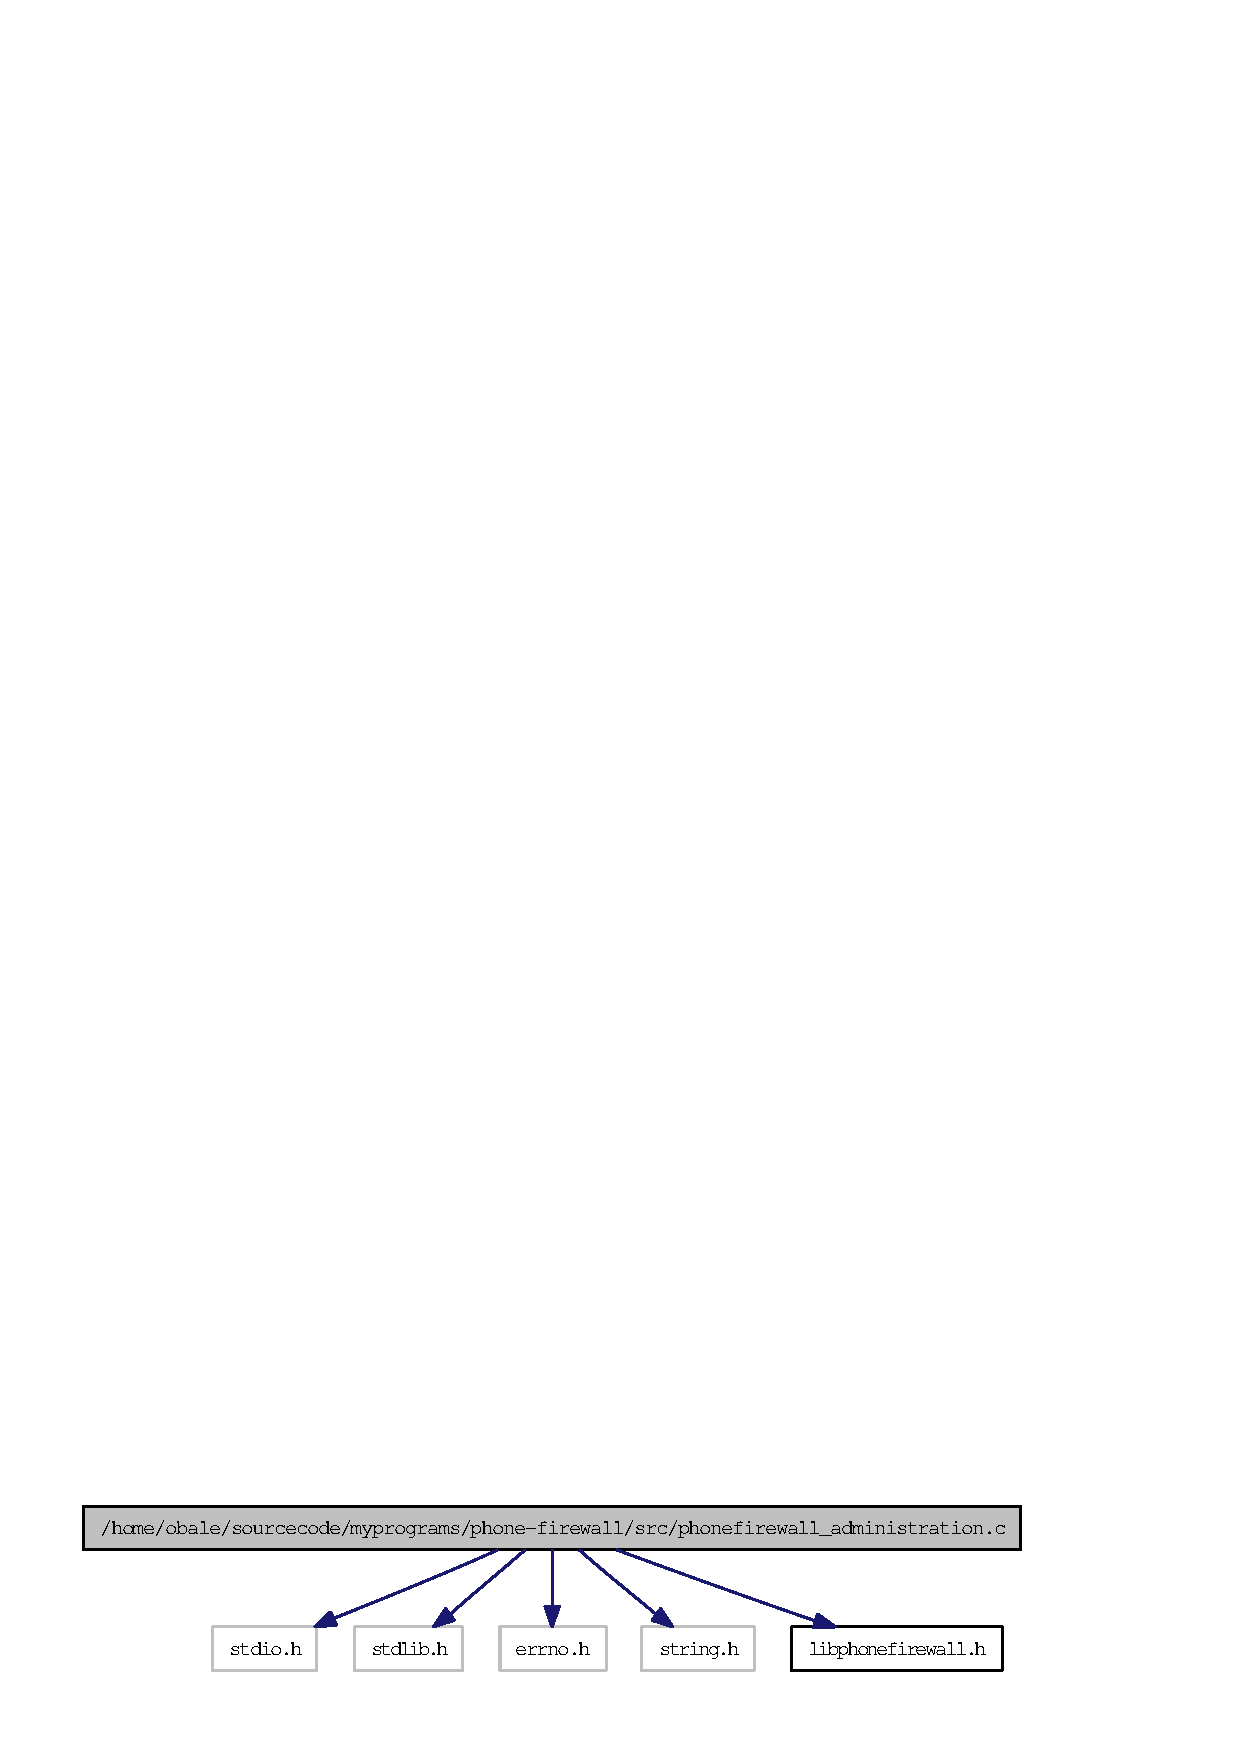
\includegraphics[width=211pt]{phonefirewall__administration_8c__incl}
\end{center}
\end{figure}
\subsection*{Defines}
\begin{CompactItemize}
\item 
\#define \hyperlink{phonefirewall__administration_8c_c0120f27d973f4ea90962305431fedce}{BLACKLIST\_\-PREFIX}~\char`\"{}db/blacklist\_\-\char`\"{}
\item 
\#define \hyperlink{phonefirewall__administration_8c_b5b8614b1e4d5e316cc4a8102ce9636c}{WHITELIST\_\-PREFIX}~\char`\"{}db/whitelist\_\-\char`\"{}
\end{CompactItemize}
\subsection*{Functions}
\begin{CompactItemize}
\item 
int \hyperlink{phonefirewall__administration_8c_ca47a7a15cc44ee9c44ccbaf61ab63b7}{add\_\-blacklist\_\-entry} (int country\_\-code, int area\_\-code, long long int number, char $\ast$name, char $\ast$reason, int priority)
\item 
int \hyperlink{phonefirewall__administration_8c_979a7b693ec5468f9caa2487bd1b7217}{add\_\-whitelist\_\-entry} (int country\_\-code, int area\_\-code, long long int number, char $\ast$name, char $\ast$reason, int priority)
\item 
int \hyperlink{phonefirewall__administration_8c_c1875490cf592d507798a292f8a772e9}{rm\_\-blacklist\_\-entry} (long long int number)
\item 
int \hyperlink{phonefirewall__administration_8c_c3a77117dbcade02ab233836e559814a}{rm\_\-whitelist\_\-entry} (long long int number)
\item 
char $\ast$ \hyperlink{phonefirewall__administration_8c_737cba40ba261f05830a454be982f56e}{check\_\-blacklist\_\-entry} (int country\_\-code, int area\_\-code, long long int number)
\item 
char $\ast$ \hyperlink{phonefirewall__administration_8c_db8b63f034438c47d82a80ed205f0ad2}{check\_\-whitelist\_\-entry} (int country\_\-code, int area\_\-code, long long int number)
\end{CompactItemize}
\subsection*{Variables}
\begin{CompactItemize}
\item 
static char $\ast$ \hyperlink{phonefirewall__administration_8c_6c7d3710dd8e86998206dad075d6fc27}{DELIM} = \char`\"{}::\char`\"{}
\end{CompactItemize}


\subsection{Define Documentation}
\hypertarget{phonefirewall__administration_8c_c0120f27d973f4ea90962305431fedce}{
\index{phonefirewall\_\-administration.c@{phonefirewall\_\-administration.c}!BLACKLIST\_\-PREFIX@{BLACKLIST\_\-PREFIX}}
\index{BLACKLIST\_\-PREFIX@{BLACKLIST\_\-PREFIX}!phonefirewall_administration.c@{phonefirewall\_\-administration.c}}
\subsubsection{\setlength{\rightskip}{0pt plus 5cm}\#define BLACKLIST\_\-PREFIX~\char`\"{}db/blacklist\_\-\char`\"{}}}
\label{phonefirewall__administration_8c_c0120f27d973f4ea90962305431fedce}




Definition at line 26 of file phonefirewall\_\-administration.c.\hypertarget{phonefirewall__administration_8c_b5b8614b1e4d5e316cc4a8102ce9636c}{
\index{phonefirewall\_\-administration.c@{phonefirewall\_\-administration.c}!WHITELIST\_\-PREFIX@{WHITELIST\_\-PREFIX}}
\index{WHITELIST\_\-PREFIX@{WHITELIST\_\-PREFIX}!phonefirewall_administration.c@{phonefirewall\_\-administration.c}}
\subsubsection{\setlength{\rightskip}{0pt plus 5cm}\#define WHITELIST\_\-PREFIX~\char`\"{}db/whitelist\_\-\char`\"{}}}
\label{phonefirewall__administration_8c_b5b8614b1e4d5e316cc4a8102ce9636c}




Definition at line 27 of file phonefirewall\_\-administration.c.

\subsection{Function Documentation}
\hypertarget{phonefirewall__administration_8c_ca47a7a15cc44ee9c44ccbaf61ab63b7}{
\index{phonefirewall\_\-administration.c@{phonefirewall\_\-administration.c}!add\_\-blacklist\_\-entry@{add\_\-blacklist\_\-entry}}
\index{add\_\-blacklist\_\-entry@{add\_\-blacklist\_\-entry}!phonefirewall_administration.c@{phonefirewall\_\-administration.c}}
\subsubsection{\setlength{\rightskip}{0pt plus 5cm}int add\_\-blacklist\_\-entry (int {\em country\_\-code}, int {\em area\_\-code}, long long int {\em number}, char $\ast$ {\em name}, char $\ast$ {\em reason}, int {\em priority})}}
\label{phonefirewall__administration_8c_ca47a7a15cc44ee9c44ccbaf61ab63b7}


Add a number to the blacklist. The number will be blocked after that.

\begin{Desc}
\item[Parameters:]
\begin{description}
\item[{\em country\_\-code}]The country code (for example 39 for Italy, 43 for Austria, and so one) \item[{\em area\_\-code}]The area code which indicates your mobile operator. \item[{\em number}]The telephone number of the person. \item[{\em name}]The name of the person. \item[{\em reason}]Why you have blocked this person. \item[{\em priority}]Has no affect at the moment. Later one it will be possible to give each number priority. So you have more control when a number will be blocked/accepted.\end{description}
\end{Desc}
\begin{Desc}
\item[Returns:]If all goes well 0 (zero) otherwise an errno code. \end{Desc}


Definition at line 31 of file phonefirewall\_\-administration.c.

References DELIM.\hypertarget{phonefirewall__administration_8c_979a7b693ec5468f9caa2487bd1b7217}{
\index{phonefirewall\_\-administration.c@{phonefirewall\_\-administration.c}!add\_\-whitelist\_\-entry@{add\_\-whitelist\_\-entry}}
\index{add\_\-whitelist\_\-entry@{add\_\-whitelist\_\-entry}!phonefirewall_administration.c@{phonefirewall\_\-administration.c}}
\subsubsection{\setlength{\rightskip}{0pt plus 5cm}int add\_\-whitelist\_\-entry (int {\em country\_\-code}, int {\em area\_\-code}, long long int {\em number}, char $\ast$ {\em name}, char $\ast$ {\em reason}, int {\em priority})}}
\label{phonefirewall__administration_8c_979a7b693ec5468f9caa2487bd1b7217}


Add a number to the whitelist. The number will be accepted after that.

\begin{Desc}
\item[Parameters:]
\begin{description}
\item[{\em country\_\-code}]The country code (for example 39 for Italy, 43 for Austria, and so one) \item[{\em area\_\-code}]The area code which indicates your mobile operator. \item[{\em number}]The telephone number of the person. \item[{\em name}]The name of the person. \item[{\em reason}]Why you have blocked this person. \item[{\em priority}]Has no affect at the moment. Later one it will be possible to give each number priority. So you have more control when a number will be blocked/accepted.\end{description}
\end{Desc}
\begin{Desc}
\item[Returns:]If all goes well 0 (zero) otherwise an errno code. \end{Desc}


Definition at line 47 of file phonefirewall\_\-administration.c.

References DELIM.\hypertarget{phonefirewall__administration_8c_737cba40ba261f05830a454be982f56e}{
\index{phonefirewall\_\-administration.c@{phonefirewall\_\-administration.c}!check\_\-blacklist\_\-entry@{check\_\-blacklist\_\-entry}}
\index{check\_\-blacklist\_\-entry@{check\_\-blacklist\_\-entry}!phonefirewall_administration.c@{phonefirewall\_\-administration.c}}
\subsubsection{\setlength{\rightskip}{0pt plus 5cm}char$\ast$ check\_\-blacklist\_\-entry (int {\em country\_\-code}, int {\em area\_\-code}, long long int {\em number})}}
\label{phonefirewall__administration_8c_737cba40ba261f05830a454be982f56e}


Checks if a number is on the blacklist.

\begin{Desc}
\item[Parameters:]
\begin{description}
\item[{\em country\_\-code}]The country code (for example 39 for Italy, 43 for Austria, and so one) \item[{\em area\_\-code}]The area code which indicates your mobile operator. \item[{\em number}]The telephone number of the person.\end{description}
\end{Desc}
\begin{Desc}
\item[Returns:]If noting is found NULL, otherwise the number. \end{Desc}


Definition at line 71 of file phonefirewall\_\-administration.c.

References DELIM, and MAX\_\-LINE\_\-LENGTH.\hypertarget{phonefirewall__administration_8c_db8b63f034438c47d82a80ed205f0ad2}{
\index{phonefirewall\_\-administration.c@{phonefirewall\_\-administration.c}!check\_\-whitelist\_\-entry@{check\_\-whitelist\_\-entry}}
\index{check\_\-whitelist\_\-entry@{check\_\-whitelist\_\-entry}!phonefirewall_administration.c@{phonefirewall\_\-administration.c}}
\subsubsection{\setlength{\rightskip}{0pt plus 5cm}char$\ast$ check\_\-whitelist\_\-entry (int {\em country\_\-code}, int {\em area\_\-code}, long long int {\em number})}}
\label{phonefirewall__administration_8c_db8b63f034438c47d82a80ed205f0ad2}


Checks if a number is on the whitelist.

\begin{Desc}
\item[Parameters:]
\begin{description}
\item[{\em country\_\-code}]The country code (for example 39 for Italy, 43 for Austria, and so one) \item[{\em area\_\-code}]The area code which indicates your mobile operator. \item[{\em number}]The telephone number of the person.\end{description}
\end{Desc}
\begin{Desc}
\item[Returns:]If noting is found NULL, otherwise the number. \end{Desc}


Definition at line 100 of file phonefirewall\_\-administration.c.

References DELIM, and MAX\_\-LINE\_\-LENGTH.\hypertarget{phonefirewall__administration_8c_c1875490cf592d507798a292f8a772e9}{
\index{phonefirewall\_\-administration.c@{phonefirewall\_\-administration.c}!rm\_\-blacklist\_\-entry@{rm\_\-blacklist\_\-entry}}
\index{rm\_\-blacklist\_\-entry@{rm\_\-blacklist\_\-entry}!phonefirewall_administration.c@{phonefirewall\_\-administration.c}}
\subsubsection{\setlength{\rightskip}{0pt plus 5cm}int rm\_\-blacklist\_\-entry (long long int {\em number})}}
\label{phonefirewall__administration_8c_c1875490cf592d507798a292f8a772e9}


Removes a blocked number from the blacklist.

\begin{Desc}
\item[Parameters:]
\begin{description}
\item[{\em number}]The number which will be deleted.\end{description}
\end{Desc}
\begin{Desc}
\item[Returns:]If all goes right 0, otherwise an error code. \end{Desc}


Definition at line 63 of file phonefirewall\_\-administration.c.\hypertarget{phonefirewall__administration_8c_c3a77117dbcade02ab233836e559814a}{
\index{phonefirewall\_\-administration.c@{phonefirewall\_\-administration.c}!rm\_\-whitelist\_\-entry@{rm\_\-whitelist\_\-entry}}
\index{rm\_\-whitelist\_\-entry@{rm\_\-whitelist\_\-entry}!phonefirewall_administration.c@{phonefirewall\_\-administration.c}}
\subsubsection{\setlength{\rightskip}{0pt plus 5cm}int rm\_\-whitelist\_\-entry (long long int {\em number})}}
\label{phonefirewall__administration_8c_c3a77117dbcade02ab233836e559814a}


Removes a accepted number from the whitelist.

\begin{Desc}
\item[Parameters:]
\begin{description}
\item[{\em number}]The number which will be deleted.\end{description}
\end{Desc}
\begin{Desc}
\item[Returns:]If all goes right 0, otherwise an error code. \end{Desc}


Definition at line 67 of file phonefirewall\_\-administration.c.

\subsection{Variable Documentation}
\hypertarget{phonefirewall__administration_8c_6c7d3710dd8e86998206dad075d6fc27}{
\index{phonefirewall\_\-administration.c@{phonefirewall\_\-administration.c}!DELIM@{DELIM}}
\index{DELIM@{DELIM}!phonefirewall_administration.c@{phonefirewall\_\-administration.c}}
\subsubsection{\setlength{\rightskip}{0pt plus 5cm}char$\ast$ {\bf DELIM} = \char`\"{}::\char`\"{}\hspace{0.3cm}{\tt  \mbox{[}static\mbox{]}}}}
\label{phonefirewall__administration_8c_6c7d3710dd8e86998206dad075d6fc27}




Definition at line 29 of file phonefirewall\_\-administration.c.

Referenced by add\_\-blacklist\_\-entry(), add\_\-whitelist\_\-entry(), check\_\-blacklist\_\-entry(), and check\_\-whitelist\_\-entry().